\documentclass[tikz,border=10pt]{standalone}
% Shared look for every TikZ diagram. Load with % Shared look for every TikZ diagram. Load with % Shared look for every TikZ diagram. Load with \input{../../tools/tikz-style.tex}
\usepackage[T1]{fontenc}
\usepackage{lmodern}
\renewcommand{\sfdefault}{lmr}  % diagrams use the same serif as the text
\usetikzlibrary{arrows.meta, positioning, shapes.geometric, calc, fit, backgrounds}
\definecolor{cblue}{HTML}{4C78A8}
\definecolor{corange}{HTML}{F58518}
\definecolor{cgreen}{HTML}{54A24B}
\definecolor{cred}{HTML}{E45756}
\definecolor{cpurple}{HTML}{B279A2}
\definecolor{cgrey}{HTML}{6B6B6B}
\tikzset{
  every picture/.style={font=\sffamily, line width=1.2pt},
  box/.style={draw=#1, fill=#1!12, rounded corners=4pt, align=center, inner sep=7pt, minimum height=1.1cm},
  box/.default=cgrey,
  arrow/.style={-{Stealth[length=3mm]}, draw=cgrey, line width=1.4pt},
  title/.style={font=\sffamily\bfseries\Large},
  note/.style={font=\sffamily\small, text=cgrey, align=center},
}
\AtBeginDocument{\hyphenpenalty=10000 \exhyphenpenalty=10000}

\usepackage[T1]{fontenc}
\usepackage{lmodern}
\renewcommand{\sfdefault}{lmr}  % diagrams use the same serif as the text
\usetikzlibrary{arrows.meta, positioning, shapes.geometric, calc, fit, backgrounds}
\definecolor{cblue}{HTML}{4C78A8}
\definecolor{corange}{HTML}{F58518}
\definecolor{cgreen}{HTML}{54A24B}
\definecolor{cred}{HTML}{E45756}
\definecolor{cpurple}{HTML}{B279A2}
\definecolor{cgrey}{HTML}{6B6B6B}
\tikzset{
  every picture/.style={font=\sffamily, line width=1.2pt},
  box/.style={draw=#1, fill=#1!12, rounded corners=4pt, align=center, inner sep=7pt, minimum height=1.1cm},
  box/.default=cgrey,
  arrow/.style={-{Stealth[length=3mm]}, draw=cgrey, line width=1.4pt},
  title/.style={font=\sffamily\bfseries\Large},
  note/.style={font=\sffamily\small, text=cgrey, align=center},
}
\AtBeginDocument{\hyphenpenalty=10000 \exhyphenpenalty=10000}

\usepackage[T1]{fontenc}
\usepackage{lmodern}
\renewcommand{\sfdefault}{lmr}  % diagrams use the same serif as the text
\usetikzlibrary{arrows.meta, positioning, shapes.geometric, calc, fit, backgrounds}
\definecolor{cblue}{HTML}{4C78A8}
\definecolor{corange}{HTML}{F58518}
\definecolor{cgreen}{HTML}{54A24B}
\definecolor{cred}{HTML}{E45756}
\definecolor{cpurple}{HTML}{B279A2}
\definecolor{cgrey}{HTML}{6B6B6B}
\tikzset{
  every picture/.style={font=\sffamily, line width=1.2pt},
  box/.style={draw=#1, fill=#1!12, rounded corners=4pt, align=center, inner sep=7pt, minimum height=1.1cm},
  box/.default=cgrey,
  arrow/.style={-{Stealth[length=3mm]}, draw=cgrey, line width=1.4pt},
  title/.style={font=\sffamily\bfseries\Large},
  note/.style={font=\sffamily\small, text=cgrey, align=center},
}
\AtBeginDocument{\hyphenpenalty=10000 \exhyphenpenalty=10000}

\begin{document}
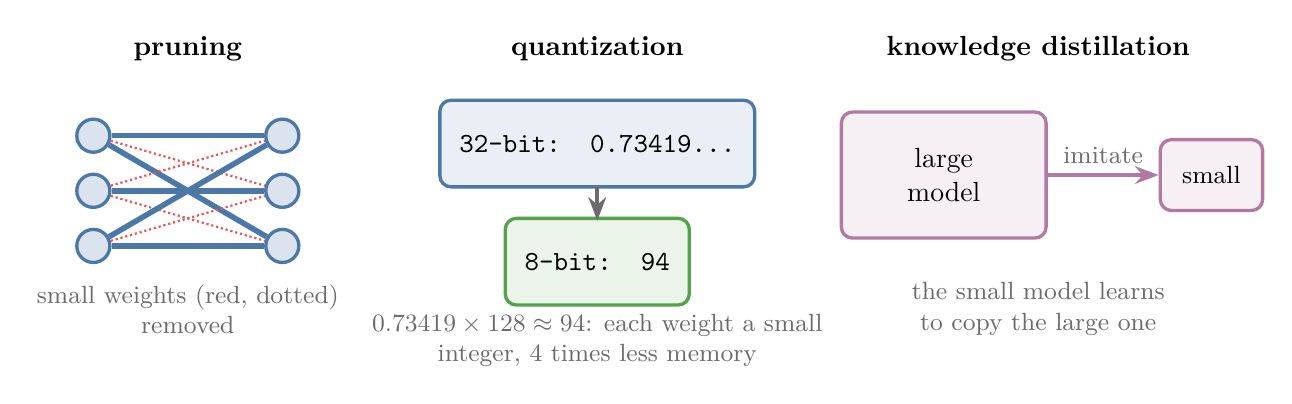
\begin{tikzpicture}[keep/.style={cblue, line width=2pt}, cut/.style={cred, densely dotted, line width=0.8pt},
  n/.style={circle, draw=cblue, fill=cblue!20, minimum size=0.42cm, inner sep=0pt}]
  % pruning
  \node[font=\sffamily\bfseries] at (1.2,2.6) {pruning};
  \foreach \i in {1,2,3} { \node[n] (a\i) at (0,2.2-0.7*\i) {}; \node[n] (b\i) at (2.4,2.2-0.7*\i) {}; }
  \foreach \i/\j/\st in {1/1/keep, 1/2/cut, 1/3/keep, 2/1/cut, 2/2/keep, 2/3/cut, 3/1/keep, 3/2/cut, 3/3/keep}
    \draw[\st] (a\i) -- (b\j);
  \node[note] at (1.2,-0.7) {small weights (red, dotted)\\removed};
  % quantization
  \node[font=\sffamily\bfseries] at (6.4,2.6) {quantization};
  \node[box=cblue, minimum width=3.6cm, font=\ttfamily] at (6.4,1.4) {32-bit: 0.73419...};
  \node[box=cgreen, minimum width=1.2cm, font=\ttfamily] at (6.4,-0.1) {8-bit: 94};
  \draw[arrow] (6.4,0.85) -- (6.4,0.42);
  \node[note] at (6.4,-1.1) {$0.73419 \times 128 \approx 94$: each weight a small\\integer, 4 times less memory};
  % distillation
  \node[font=\sffamily\bfseries] at (12.0,2.6) {knowledge distillation};
  \node[box=cpurple, minimum width=2.6cm, minimum height=1.6cm] (big) at (10.8,1.0) {large\\model};
  \node[box=cpurple, minimum width=1.3cm, minimum height=0.9cm, font=\sffamily\small] (small) at (14.2,1.0) {small};
  \draw[arrow, draw=cpurple] (big) -- node[above, note] {imitate} (small);
  \node[note] at (12.0,-0.7) {the small model learns\\to copy the large one};
\end{tikzpicture}
\end{document}
